\documentclass[12pt, a4paper]{article}

\usepackage{graphicx}
\usepackage{float}
\usepackage{hyperref}
\usepackage{siunitx}

\begin{document}
	\pagenumbering{gobble}
		\begin{titlepage}
			\centering
			{\LARGE Controls Systems Practical 3 \par}
			\vspace*{1.5cm}
			{\large Q. Kruger, 216008466 \par}
			{\large R. de Bruyn, 216054484 \par}
			\vspace*{1.2cm}
			{\large \today}
			\vspace*{\fill}
			% 
\includegraphics[width=\textwidth]{img/UJ.jpg}
			\vspace*{\fill}
		\end{titlepage}

		\pagenumbering{roman}
		\tableofcontents
		\listoffigures
		\listoftables
		\newpage
		\pagenumbering{arabic}

	\section{Prelab} % (fold)
	\label{sec:prelab}
		\subsection{Question 1a} % (fold)
		\label{sub:question_1}
		The transfer function of interest is 

		\begin{equation}
			\label{eqn:G_1}
			G_1(s) =\frac{25}{s^2 +4s+25} \\
		\end{equation}
				
	
		This equation shows that the natural frequency $\omega_n$ is given as $\omega_n = 5$ and zeta is given as $\zeta = 0.8$\\ 

		Using the value for $\zeta$ and $\omega_n$ the rise time ($T_r$), settling time ($T_s$), peak time ($T_p$) and persent overshoot ($\%OS$)can be found using the respective equations:
		\[
			\begin{array}{rcl}

				T_r &=& \frac{1}{\omega_n}(1.763\zeta^3-0.147\zeta^2+1.039\zeta+1)\\
				T_s &=& \frac{4}{\zeta\omega_n}\\
				T_p &=& \frac{\pi}{\omega_n\sqrt{1-\zeta^2}}\\
				\%OS &=& e^{-(\frac{\zeta\pi}{\sqrt{1-\zeta^2}})} \times 100\\
				\\
				T_r &=& 0.493 s \\
				T_p &=& 1.05 s\\
				T_s &=& 1 s\\
				\%OS &=& 1.5 \%\\
			\end{array}
		\]

		The pole plot for the transfer function as given by equation \ref{eqn:G_1} is shown in Figure \ref{fig:pole_plot_pre_g1a} below

		\begin{figure}[H]
			\centering
				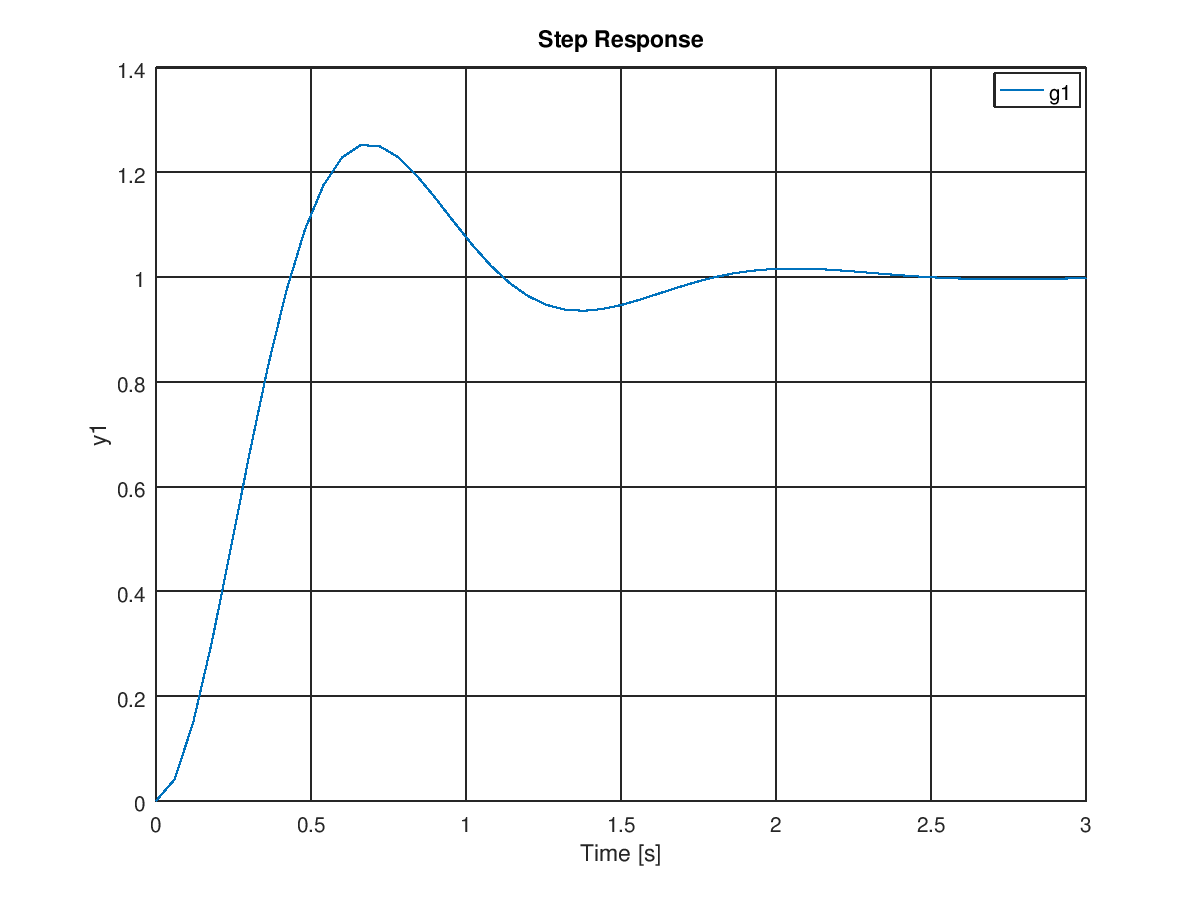
\includegraphics[width=0.7\textwidth]{Images/pole_plot_pre_q1a.png}
				\caption{Pole plot for $G_1$}
				\label{fig:pole_plot_pre_g1a} 
		\end{figure}

		\subsection{Question 1b} % (fold)
		\label{sub:question_1b}
			Consider an addtional pole at $s=-200$. The new transfer function is given shown by equation \ref{}
			\begin{equation}
				G_2 = \frac{25}{s^3+204s^2+825s+5000}
			\end{equation}

			Comparing the transfer function $G_1$ with that of $G_2$, the additonal pole chnaged the gain of the system as can be seen from the 2 figures showing the step response of $G_1$ and $G_2$ respectively (Figure \ref{fig:pole_plot_pre_q1b_step_g1} and \ref{fig:pole_plot_pre_q1b_step_g2})

			\begin{figure}[H]
				\centering
				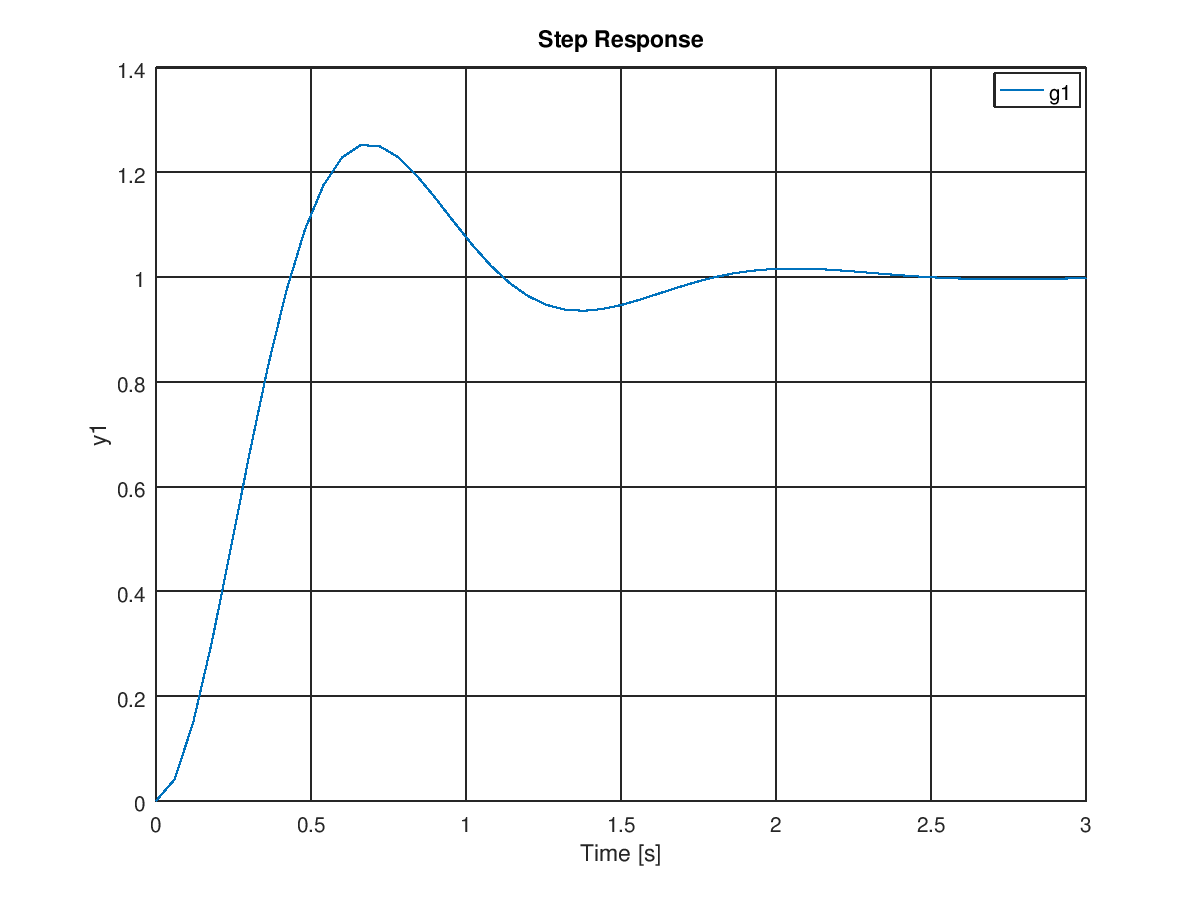
\includegraphics[width=0.7\textwidth]{Images/pole_plot_pre_q1b_step_g1.png}
				\caption{Step response of the system with transfer function $G_1$}
				\label{fig:pole_plot_pre_q1b_step_g1}
			\end{figure}

			\begin{figure}[H]
				\centering
				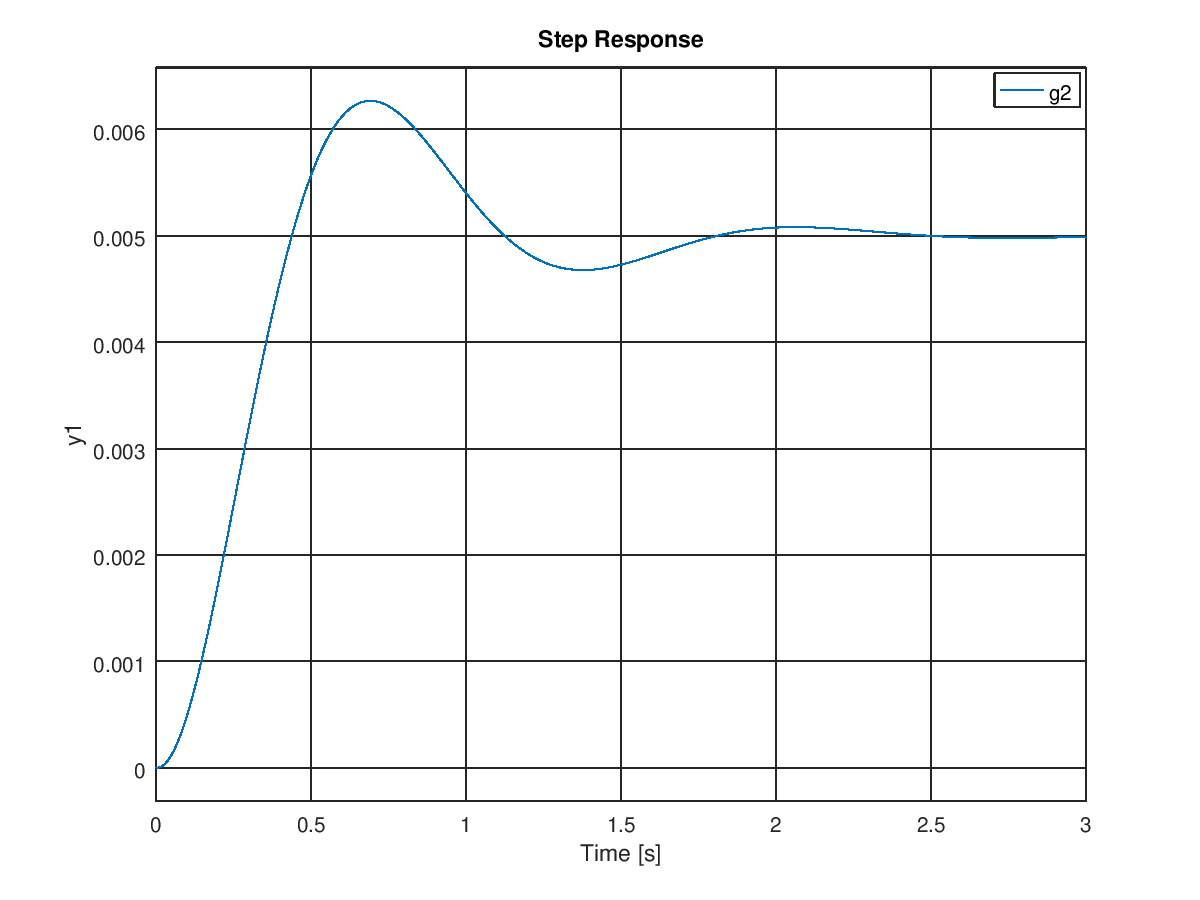
\includegraphics[width=0.7\textwidth]{Images/pole_plot_pre_q1b_step_g2.png}
				\caption{Step response of the system with transfer function $G_2$}
				\label{fig:pole_plot_pre_q1b_step_g2}
			\end{figure}


		
		% subsection question_1b (end)




		
		% subsection question_1 (end)
	
	% section prelab (end)

\end{document}

